\documentclass[border=0.2cm]{standalone}
 
% Required packages
\usepackage[dvipsnames]{xcolor}
\usepackage{tikz}
 
 
\begin{document}

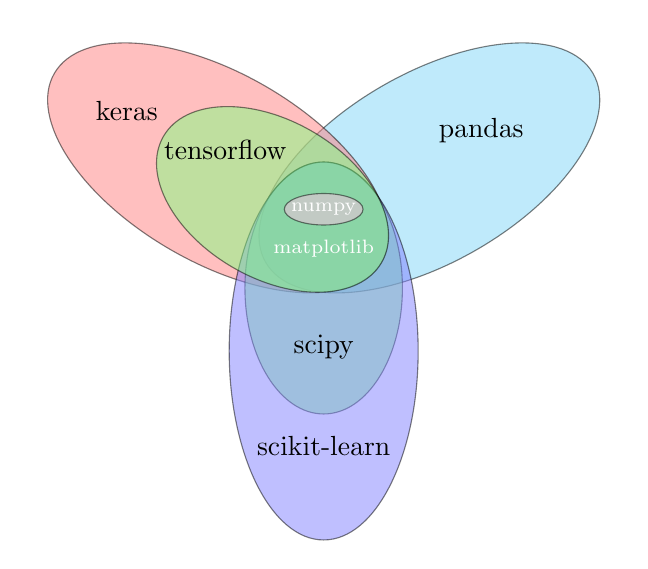
\begin{tikzpicture} 

\draw[fill=cyan!50!white, rotate=30, opacity = 0.5] (1.55, 0) ellipse (24mm and 12mm);
\draw[fill=red!50!white, rotate=150, opacity = 0.5] (1.55, 0) ellipse (24mm and 12mm);
\draw[fill=green!50!white, rotate=270, opacity = 0.5] (0.75, 0) ellipse (16mm and 10mm);
\draw[fill=blue!50!white, rotate=270, opacity = 0.5] (1.55, 0) ellipse (24mm and 12mm);
\draw[fill=green!50!white, rotate=150, opacity = 0.5] (0.75, 0) ellipse (16mm and 10mm);
\draw[fill=magenta!25!white, rotate=0, opacity = 0.5] (0, 0.25) ellipse (5mm and 2mm);  % numpy

\node at (0, 0.25) [text=white, font=\scriptsize] {numpy};
\node at (0, -0.25) [text=white, font=\scriptsize] {matplotlib};
\node at (2.0, 1.25) [text=black] {pandas};
\node at (0, -1.5) [text=black] {scipy};
\node at (0, -2.75) [text=black] {scikit-learn};
\node at (-1.25, 1.0) [text=black] {tensorflow};
\node at (-2.5, 1.5) [text=black] {keras};
\end{tikzpicture}
 
 
\end{document}